% ============================================================
% CHAPITRE 5
% ============================================================
\chapter{Détection : du motif au score expliqué}
\label{ch:algorithmes}

\section{Chemin rapide : ne chercher que là où une boucle peut naître}
Rechercher le motif \fichier{(a)-[e1]->(b); (b)-[e2]->(c); (c)-[e3]->(a)} sur
tout le graphe glissant à chaque micro-batch revient à joindre trois fois une
table de 36\,000 arêtes avec elle-même, alors que presque rien n'a changé
depuis le lot précédent. Or une boucle \emph{nouvelle} contient forcément une
arête nouvelle. Pour une arête nouvelle $u \to v$, il suffit donc de trouver
les comptes $w$ qui reçoivent de $v$ et envoient à $u$
(figure~\ref{fig:triangle}). L'index d'adjacence en mémoire répond à cette
question par une simple intersection d'ensembles.

\begin{figure}[htp]
\centering
\begin{tikzpicture}
  \begin{scope}
    \node[compteo] (u) at (0,0) {u};
    \node[compteo] (v) at (3.0,0) {v};
    \draw[virement, color=orangeprojet, line width=1.6pt] (u) -- node[montant, above=1pt, fill=none] {arête nouvelle} (v);
    \node[compteg] (w1) at (4.5,1.2) {w\textsubscript{1}};
    \node[compteg] (w2) at (1.5,-1.75) {w\textsubscript{2}};
    \node[compteg] (w3) at (4.6,-1.3) {w\textsubscript{3}};
    \node[compteg] (w4) at (-1.5,-1.3) {w\textsubscript{4}};
    \draw[virement, color=grismoyen] (v) -- (w1);
    \draw[virement, color=bleuprojet, line width=1.3pt] (v) -- (w2);
    \draw[virement, color=grismoyen] (v) -- (w3);
    \draw[virement, color=bleuprojet, line width=1.3pt] (w2) -- (u);
    \draw[virement, color=grismoyen] (w4) -- (u);
    \node[font=\sffamily\tiny, color=encre2, align=center] at (1.5,-0.55) {triangle\\fermé};
  \end{scope}
  \begin{scope}[xshift=7.6cm, yshift=0.9cm]
    \node[anchor=north west, text width=7.2cm, font=\sffamily\scriptsize, align=left] at (0,0) {
      \textbf{Pour chaque arête nouvelle} $u \to v$ du lot :\\[3pt]
      \quad sorties de $v$ \hspace{2pt}= \{w\textsubscript{1}, w\textsubscript{2}, w\textsubscript{3}\}\\
      \quad entrées de $u$ = \{w\textsubscript{2}, w\textsubscript{4}\}\\
      \quad intersection \hspace{3pt}= \{\textbf{\color{bleuprojet}w\textsubscript{2}}\}
        $\Rightarrow$ arêtes candidates : $u{\to}v$, $v{\to}w_2$, $w_2{\to}u$\\[5pt]
      {\color{encre2}Coût proportionnel au lot et au degré des comptes concernés, pas à la taille
      du graphe. Le motif GraphFrames est ensuite exécuté sur ces seules arêtes, pour garder la
      sémantique de l'énoncé et vérifier l'ordre temporel.}};
  \end{scope}
\end{tikzpicture}
\caption{Élagage incrémental : seules les arêtes qui ferment un triangle avec une arête nouvelle
sont transmises au motif.}
\label{fig:triangle}
\end{figure}

L'effet est spectaculaire (figure~\ref{fig:elagage}) : le motif ne voit plus
qu'une centaine d'arêtes par lot au lieu de plusieurs dizaines de milliers.
C'est ce qui a fait passer le motif de 68~secondes à 0,73~seconde
(chapitre~\ref{ch:performance}).

\begin{figure}[htp]
\centering
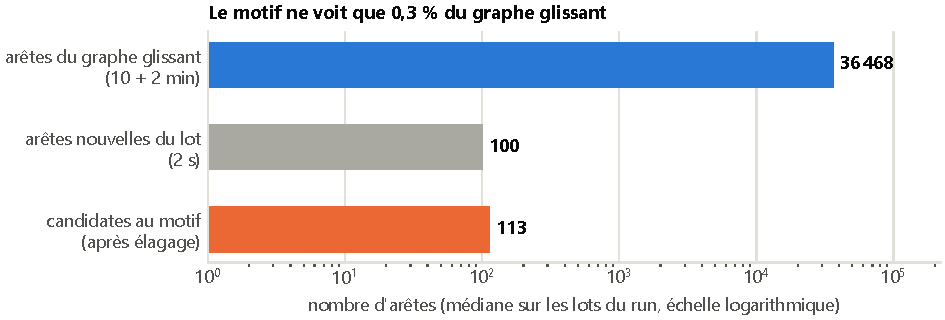
\includegraphics[width=\linewidth]{figures/elagage_candidats.pdf}
\caption[Effet de l'élagage incrémental]{Effet de l'élagage incrémental, rejoué lot par lot (lots de
2~s) sur les transactions du run : médianes sur 998 lots.}
\label{fig:elagage}
\end{figure}

\section{L'ordre temporel : une boucle doit être parcourue dans le temps}
Le motif trouve tout triangle orienté, y compris des boucles fortuites entre
commerçants où le « retour » a eu lieu \emph{avant} l'« aller ». Une boucle de
blanchiment, elle, est parcourue dans l'ordre : l'argent quitte $a$, passe
par $b$ puis $c$, et revient. La détection impose donc
$t(e_1) < t(e_2) < t(e_3)$ et une durée totale d'au plus 10~minutes. Cette
contrainte a un second effet utile : chacun des trois « tours » du même
triangle ($abc$, $bca$, $cab$) que renvoie le motif n'est retenu qu'une fois,
celui qui commence par le virement le plus ancien (figure~\ref{fig:temporel}).

\begin{figure}[htp]
\centering
\begin{tikzpicture}[
  mini/.style={circle, fill=#1, text=white, minimum size=5.5mm, inner sep=0pt, font=\sffamily\tiny\bfseries},
  t/.style={font=\sffamily\tiny, fill=white, inner sep=1pt}]
  \foreach \x/\o/\ok/\lab in {0/abc/1/{$t_1<t_2<t_3$ : retenu}, 4.1/bca/0/{$t_2<t_3$ mais $t_3 \not< t_1$ : écarté}, 8.2/cab/0/{$t_3 \not< t_1$ : écarté}} {
    \begin{scope}[xshift=\x cm]
      \ifnum\ok=1 \def\coul{orangeprojet}\else\def\coul{grismoyen}\fi
      \node[mini=\coul] (a) at (90:0.8) {a};
      \node[mini=\coul] (b) at (-30:0.8) {b};
      \node[mini=\coul] (c) at (210:0.8) {c};
      \draw[virement, color=\coul, bend left=18] (a) to node[t] {$t_1$} (b);
      \draw[virement, color=\coul, bend left=18] (b) to node[t] {$t_2$} (c);
      \draw[virement, color=\coul, bend left=18] (c) to node[t] {$t_3$} (a);
      \node[font=\sffamily\scriptsize\bfseries] at (0,1.35) {motif lu depuis {\ttfamily \o}};
      \node[font=\sffamily\tiny, color=encre2, text width=3.5cm, align=center] at (0,-1.25) {\lab};
    \end{scope}
  }
  \begin{scope}[xshift=12.3cm]
    \node[mini=grismoyen] (a) at (90:0.8) {a};
    \node[mini=grismoyen] (b) at (-30:0.8) {b};
    \node[mini=grismoyen] (c) at (210:0.8) {c};
    \draw[virement, color=grismoyen, bend left=18] (a) to node[t] {10:05} (b);
    \draw[virement, color=grismoyen, bend left=18] (b) to node[t] {10:07} (c);
    \draw[virement, color=grismoyen, bend left=18] (c) to node[t] {09:58} (a);
    \node[font=\sffamily\scriptsize\bfseries] at (0,1.35) {boucle fortuite};
    \node[font=\sffamily\tiny, color=encre2, text width=3.2cm, align=center] at (0,-1.25) {le « retour » précède l'« aller » : aucun tour n'est ordonné};
  \end{scope}
\end{tikzpicture}
\caption{Le filtre temporel retient exactement un tour de chaque vraie boucle et aucune boucle
fortuite.}
\label{fig:temporel}
\end{figure}

\section{Un score expliqué plutôt qu'une boîte noire}
Chaque boucle retenue reçoit un score de 0 à 100, somme de règles
indépendantes qui traduisent la signature d'un carrousel
(tableau~\ref{tab:score}). Chaque règle déclenchée produit une phrase, et
l'explication complète accompagne l'alerte jusque dans Kafka, Delta et le
tableau de bord. Les niveaux sont LOW ($\geq$\,20), MEDIUM ($\geq$\,40),
HIGH ($\geq$\,70) et CRITICAL ($\geq$\,90) ; seules les alertes de niveau
MEDIUM et plus sont publiées dans Kafka, toutes sont historisées.

\begin{table}[htp]
\centering\small
\begin{tabular}{@{}>{\raggedright\arraybackslash}p{5.2cm}>{\raggedright\arraybackslash}p{6.2cm}r@{}}
\toprule
\sffamily\bfseries Règle (cycles) & \sffamily\bfseries Condition & \sffamily\bfseries Points\\
\midrule
Montants quasi identiques & écart max $\leq$ 10\,\% (proches : $\leq$ 25\,\%) & 30 (15)\\
Commission régulière & perte de 0,2 à 6\,\% à \emph{chaque} étape & 15\\
Boucle rapide & bouclée en $\leq$ 5 min ($\leq$ 10 min) & 20 (10)\\
Montants élevés & $\geq$ 100\,000 MAD ($\geq$ 30\,000 ; $\geq$ 10\,000) & 15 (10 ; 5)\\
Même type d'opération & sur toute la boucle & 5\\
Compte pivot & PageRank dans le top 1\,\% (top 5\,\%) & 10 (5)\\
Cycle long & 4 sauts ou plus & 5\\
\bottomrule
\end{tabular}
\caption[Règles du score des cycles]{Règles du score des cycles (\fichier{fraud/scoring.py}). Les
mules, scatter-gather et pivots ont leurs propres grilles, construites de la même façon.}
\label{tab:score}
\end{table}

\begin{figure}[htp]
\centering
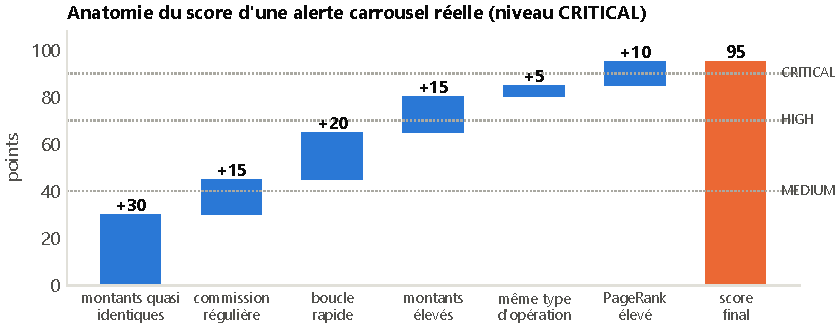
\includegraphics[width=\linewidth]{figures/score_carrousel.pdf}
\caption[Anatomie du score d'une alerte réelle]{Anatomie du score de l'alerte de la
figure~\ref{fig:carrousel}, telle qu'elle a été publiée dans Kafka.}
\label{fig:score}
\end{figure}

\begin{tcolorbox}[colback=grisclair, colframe=orangeprojet, boxrule=0pt, leftrule=3pt, arc=0pt,
  outer arc=0pt, left=8pt, right=8pt, top=5pt, bottom=5pt]
{\sffamily\bfseries\scriptsize\color{orangeprojet}ALERTE CYCLE · score 95 · CRITICAL · latence 7,0~s}\par\smallskip
\small\sffamily ACC-2801 → ACC-1853 → ACC-2052 → ACC-2801 en 2 min 27 s, 3 virements de 126\,436 MAD à
133\,500 MAD, 94,7\,\% du montant revient à l'origine. Indices : montants quasi identiques à chaque
étape (écart max 5,6\,\%) (+30) ; perte régulière de 2,7\,\% par étape (commission typique d'un
carrousel) (+15) ; boucle bouclée en 2 min 27 s (+20) ; montants élevés ($\geq$ 100\,000 MAD) (+15) ;
même type d'opération sur toute la boucle (+5) ; un compte du cycle est un pivot du réseau
(PageRank élevé) (+10).
\end{tcolorbox}

\section{Chemin lent : analyser toute la fenêtre}
Toutes les 90~secondes, le chemin lent relit dans la table bronze les
10~dernières minutes de transactions et enchaîne cinq analyses
(figure~\ref{fig:cheminlent}).

\begin{figure}[htp]
\centering
\begin{tikzpicture}[
  b/.style={draw=#1, line width=0.8pt, fill=#1!8, rounded corners=3pt, align=center,
    font=\sffamily\tiny, text width=2.25cm, minimum height=0.95cm, inner sep=2pt},
  lourd/.style={dashed, line width=1pt},
  sortie/.style={rounded corners=2pt, fill=#1, text=white, font=\sffamily\tiny\bfseries, inner sep=3pt, anchor=west},
  f/.style={-{Stealth[length=1.6mm]}, line width=0.6pt, color=encre2}]
  \node[b=bleuprojet, text width=1.9cm, minimum height=5.0cm] (win) at (0,0.55) {\textbf{fenêtre de 10 min}\\lue dans le bronze\\[3pt]$\approx$\,30\,000 arêtes};
  % gros flux
  \node[b=grismoyen] (hv) at (2.85,1.95) {\textbf{graphe des gros flux}\\$\geq$ 20\,000 MAD\\$\approx$\,2\,500 arêtes};
  % ligne A : PageRank, pivots, CC
  \node[b=bleuprojet, lourd] (pr) at (5.6,2.6) {\textbf{PageRank}\\10 itérations};
  \node[b=cat2] (pv) at (8.35,2.6) {\textbf{pivots}\\comptes dans $\geq$ 2 cycles récents};
  \node[b=cat6] (cc) at (11.1,2.6) {\textbf{Connected Components}\\comptes déjà alertés};
  % ligne B : élagage, SCC, motifs longs
  \node[b=bleuprojet, lourd] (tr) at (5.6,1.25) {\textbf{élagage} (4 tours)\\comptes sans entrée ou sans sortie retirés};
  \node[b=bleuprojet, lourd] (scc) at (8.35,1.25) {\textbf{SCC}\\sur le noyau ($\approx$\,40 arêtes)};
  \node[b=bleuprojet, lourd] (lc) at (11.1,1.25) {\textbf{motifs 4 et 5}\\dans les SCC de 4 comptes et +};
  % ligne C : mules
  \node[b=cat5] (dl) at (2.85,-0.1) {\textbf{journal des dépôts}\\40 min, en mémoire};
  \node[b=cat5] (mu) at (5.6,-0.1) {\textbf{rafale + vidage}\\rythme $\geq$ 3$\times$ l'habituel};
  % ligne D : scatter-gather
  \node[b=cat4] (sg) at (5.6,-1.35) {\textbf{motif à 2 sauts}\\\fichier{(s)->(m)->(t)}};
  % sorties
  \node[sortie=cat2] at ($(pv.south east)+(-0.75,-0.33)$) {PIVOT};
  \node[sortie=cat6] at ($(cc.east)+(0.12,0)$) {CLUSTER};
  \node[sortie=cat3] at ($(lc.east)+(0.12,0)$) {CYCLE\_LONG};
  \node[sortie=cat5] at ($(mu.east)+(0.12,0)$) {MULE};
  \node[sortie=cat4] at ($(sg.east)+(0.12,0)$) {SCATTER\_GATHER};
  % flux
  \draw[f] (win.east |- hv) -- (hv);
  \draw[f] (hv.east) -- (pr.west);
  \draw[f] (hv.east) -- (tr.west);
  \draw[f] (pr) -- (pv);
  \draw[f] (pv) -- (cc);
  \draw[f] (tr) -- (scc);
  \draw[f] (scc) -- (lc);
  \draw[f] (win.east |- dl) -- (dl);
  \draw[f] (dl) -- (mu);
  \draw[f] (win.east |- sg) -- (sg);
  \draw[f, dashed] ($(pv.north)+(0,0.55)$) node[above, font=\sffamily\tiny, color=encre2] {alertes CYCLE du chemin rapide} -- (pv.north);
  % légende
  \draw[bleuprojet, dashed, line width=1pt, rounded corners=2pt] (8.0,-0.55) rectangle (8.5,-0.25);
  \node[font=\sffamily\tiny, anchor=west, text width=4.2cm] at (8.6,-0.4) {analyse « lourde » : un passage sur deux};
\end{tikzpicture}
\caption[Les analyses du chemin lent]{Les analyses du chemin lent et les types d'alertes qu'elles
produisent. Les analyses en pointillés ne s'exécutent qu'un passage sur deux.}
\label{fig:cheminlent}
\end{figure}

\subsection*{Cycles longs : élaguer avant de chercher}
Un cycle ne peut passer que par des comptes qui reçoivent \emph{et} envoient.
Retirer itérativement les comptes sans entrée ou sans sortie réduit le graphe
des gros flux à un petit noyau, sur lequel les composantes fortement
connexes (SCC) sont calculées ; le motif à 4 ou 5 arêtes n'est cherché
qu'à l'intérieur des SCC d'au moins quatre comptes (figure~\ref{fig:grosflux}).

\begin{figure}[htp]
\centering
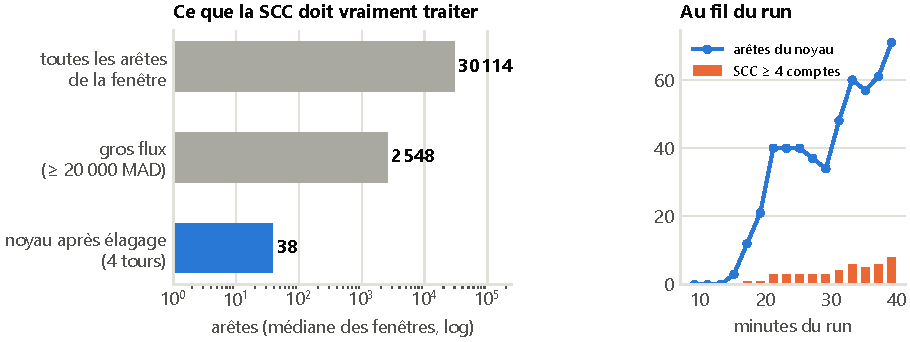
\includegraphics[width=\linewidth]{figures/elagage_gros_flux.pdf}
\caption[Réduction du graphe avant la SCC]{Réduction du graphe avant le calcul des SCC, recalculée
toutes les 2~minutes du run. Le noyau grossit au fil des fraudes injectées : il ne contient presque
que des schémas de blanchiment.}
\label{fig:grosflux}
\end{figure}

\subsection*{PageRank : un pivot n'est pas un hub}
PageRank seul désigne surtout\ldots{} les commerçants : ils reçoivent de
partout. La figure~\ref{fig:pagerank} le montre sur le dernier instantané du
run : sur les 15 comptes au plus fort PageRank, 8 sont des hubs légitimes. La
plateforme ne déclenche donc jamais d'alerte sur le PageRank seul : un compte
devient PIVOT s'il participe à au moins deux cycles suspects récents, et son
PageRank vient seulement renforcer le score.

\begin{figure}[htp]
\centering
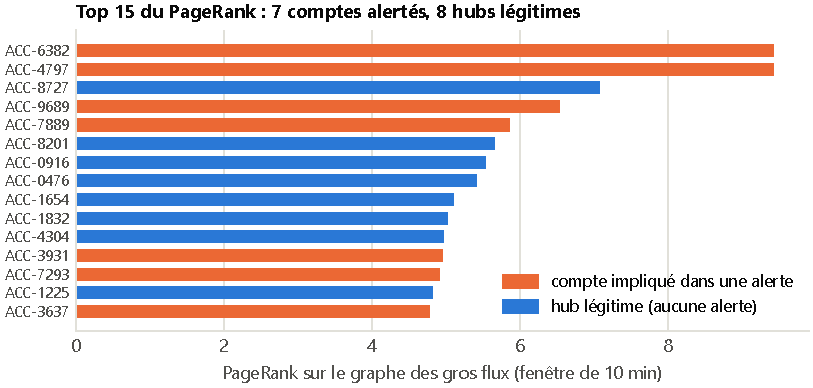
\includegraphics[width=\linewidth]{figures/pagerank_top.pdf}
\caption[PageRank : comptes alertés et hubs légitimes]{Les 15 comptes au plus fort PageRank du graphe des
gros flux à la fin du run : la moitié sont des hubs légitimes, d'où la règle combinée.}
\label{fig:pagerank}
\end{figure}

\subsection*{Comptes mules : la vélocité plutôt que le volume}
Un commerçant reçoit lui aussi beaucoup de petits paiements de nombreux
émetteurs. Ce qui distingue une mule, c'est le \emph{changement de rythme}
d'un compte habituellement calme, suivi d'un vidage. La règle finale, issue
de cinq versions mesurées contre la vérité terrain, retient un compte si,
dans les 6~minutes qui précèdent son plus gros virement sortant, il a reçu
d'au moins 6 émetteurs au moins 30\,000~MAD, à un rythme au moins trois fois
supérieur à son rythme des 20~minutes précédentes, et que ce virement unique
reprend 75 à 102\,\% des dépôts (figure~\ref{fig:mule}).

\begin{figure}[htp]
\centering
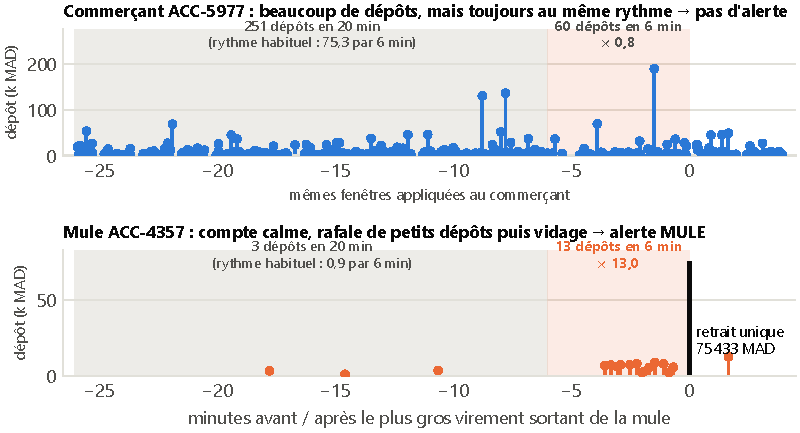
\includegraphics[width=\linewidth]{figures/mule_velocite.pdf}
\caption[Mule et commerçant face à la règle de vélocité]{La règle de vélocité appliquée à une mule
réellement détectée pendant le run et au commerçant le plus payé. Le commerçant reçoit bien plus de
dépôts, mais à son rythme habituel ($\times$\,0,8) ; la mule, elle, passe de presque rien à 13 dépôts
en 6~minutes ($\times$\,13).}
\label{fig:mule}
\end{figure}

\lecon{Ce que les versions précédentes ont appris}{Sans le critère de rythme habituel, 18 commerçants
étaient signalés comme mules. Sans la restriction aux dépôts \emph{précédant} le retrait, des dépôts
légitimes postérieurs diluaient la rafale et cachaient de vraies mules. Les deux ensemble ont fait
passer la règle de 5 mules trouvées sur 6 avec 18 fausses alertes à 12 sur 15 sans aucune fausse
alerte.}

\subsection*{Réseaux : relier les alertes}
Un pivot relie plusieurs carrousels ; plusieurs schémas peuvent partager des
comptes. Les \textbf{Connected Components} sont calculées sur le sous-graphe
des seuls comptes déjà alertés : chaque composante qui rassemble plusieurs
alertes devient une alerte CLUSTER, qui donne à l'analyste la vue d'ensemble
du réseau (figure~\ref{fig:reseau}).

\begin{figure}[htp]
\centering
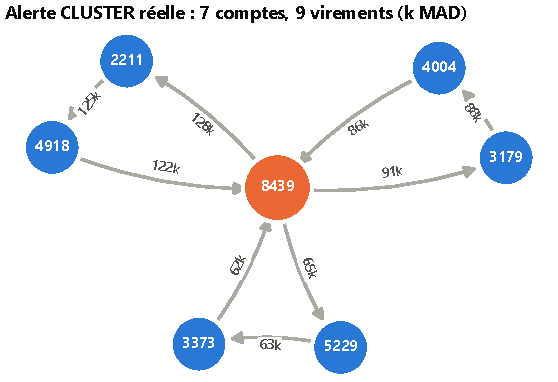
\includegraphics[width=0.78\linewidth]{figures/reseau_cluster.pdf}
\caption[Une alerte CLUSTER réelle]{Une alerte CLUSTER réelle du run : le compte ACC-8439 (en orange)
est au centre de trois carrousels imbriqués, injectés comme un seul scénario PIVOT.}
\label{fig:reseau}
\end{figure}

\section{Vue d'ensemble des alertes produites}
La figure~\ref{fig:scorestypes} place les 111 alertes de la période évaluée
selon leur type et leur score. Les fausses alertes sont presque toutes des
boucles fortuites de niveau LOW, conservées dans Delta pour l'audit mais
jamais publiées ; une seule a atteint le niveau MEDIUM.

\begin{figure}[htp]
\centering
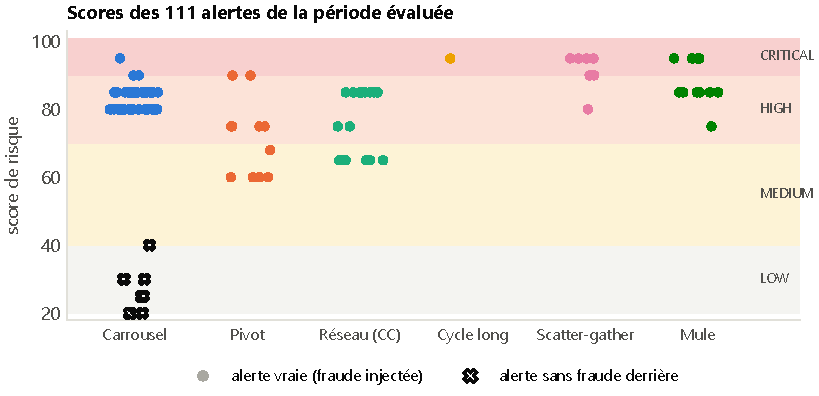
\includegraphics[width=\linewidth]{figures/scores_par_type.pdf}
\caption[Scores des alertes par type]{Score de chaque alerte de la période évaluée, par type, confronté à la
vérité terrain. Les croix sont les alertes qui ne correspondent à aucune fraude injectée.}
\label{fig:scorestypes}
\end{figure}
